\documentclass[a4paper,12pt]{article}
\usepackage{jheppub} % for details on the use of the package, please see the JINST-author-manual
\usepackage{lineno}
\usepackage{indentfirst}
\usepackage{subcaption} % Add this for subfigure environment
\usepackage{float} % Add this for the [H] float placement option

% \linenumbers



% \arxivnumber{1234.56789} % if you have one

\title{QIC Final Project: Anisotropic Transmission of quantum information through quantum fields}

% Collaborations

%% [A] If main author
%% \collaboration{\includegraphics[height=17mm]{collabroation-logo}\\[6pt]
%%  XXX collaboration}

%% or
%% [B] If "on behalf of"
%% \collaboration[c]{on behalf of XXX collaboration}


% Authors
% The "\note" macro will give a warning: "Ignoring empty anchor...", you can safely ignore it.

%% [A] simple case: 2 authors, same institution
%% \author[1]{A. Uthor\note{Corresponding author.}}
%% \author{and A. Nother Author}
%% \affiliation{Institution,\\Address, Country}

%% or, e.g.
%% [B] more complex case: 4 authors, 3 institutions, 2 footnotes
%% \author[a,b]{F. Irst,\note{Now at another university}}
%% \author[c]{S. Econd,}
%% \author[a,2]{T. Hird\note{Also at Some University.}}
%% \author[c,2]{and Fourth}
%% \affiliation[a]{Institution_1,\\Address, Country}
%% \affiliation[b]{Institution_2,\\Address, Country}
%% \affiliation[c]{Institution_3,\\Address, Country}

\author{T. Hsu}
\affiliation{National Taiwan University,\\
Taipei, Taiwan}
% \affiliation{Another University,\\
% different-address, Country}

% E-mail addresses: only for the corresponding author
\emailAdd{b11901097@ntu.edu.tw}

\abstract{In this letter, we briefly review the possible way to transmit the quantum information via quantum fields \cite{PhysRevD.101.036014}, and then we discuss }



\begin{document}
\maketitle
\flushbottom
% \section{Path Integral in Euclidean Signature}
\section{Quantum Channel: Via Quantum Mechanics}
In quantum information theory, the information is represented by a qubit, and it can be transformed, projected, and transmitted based on basic quantum mechanics postulates.
In this letter, we focus on the transmission of a qubit from a spacetime emitter Alice $ A $ to a receiver Bob $ B $.

There are various ways to transmit a qubit without contacting, which are based on the \textit{resources} Alice and Bob share.
For instance, if an entangled state is shared, they can transmit the qubit by Alice performing the Bell measurement and then send the result (a classical cbit) to Bob, which is the well-known \textit{quantum teleportation}.
Here, we simply consider transmission by a third quantum bit $ C $, $ \hat \rho_{ C, 0 } $.
Denote Alice's qubit as $ \hat \rho_{ A, 0 } $ and Bob's qubit $ \hat \rho_{ B, 0 }$; the transmission is done by performing SWAP between $ A $ and $ C $, and then between $ C $ and $ B $. 
The whole process is unitary and does not violate the non-cloning process because Alice's qubit becomes $ \hat \rho_{ C, 0 } $.

The SWAP operator can be derived by assuming $ \hat \rho_{ C, 0 } = | 0 \ar \al 0 |$ and $ \hat \rho_{ A, 0 } = | a \ar \al a | $ with $ \al a | 0 \ar \ne 0 $, and $ | a \ar = \alpha | 0 \ar + \beta | 1 \ar $:
\be
    U \rho_{ A, 0 } \otimes \rho_{ C, 0 } U^{\dagger} = \rho_{ C, 0 } \otimes \rho_{ A, 0 }
\ee

The SWAP operator is:
\be
    U = \begin{pmatrix}
        1 & 0 & 0 & 0\\
        0 & \alpha^* & \beta^* & 0\\
        0 & \beta & -\alpha & 0\\
        0 & 0 & 0 & 1\\
    \end{pmatrix}
\ee

\textbf{Remark: }
The transmission of qubit described above is rather trivial; however, it is based on an important fact that the dimension of the Hilbert space of $ C $ is the same as those of the Hilbert space of $ A $ and $ B $, so there is an isomorphism between the Hilbert spaces.
As we will see in the next section, the Hilbert space (or more precisely, the Fock space) of quantum fields is infinite-dimensional, and therefore there is no isomorphism like SWAP gate in the quantum mechanic case.

\section{Quantum Channel: Via Quantum Fields}
In this section, we briefly review the idea of quantum transmission via quantum fields \cite{PhysRevD.101.036014}.
As we will see, quantum field theory generally provides a physical picture of transmission and is consistent with the principles of special relativity.

\subsection*{Brief Review on Quantum Field Theory}
Many quantum field theory textbooks introduce the quantum field by analog of harmonic oscillators, and here we follow the same logic.
The equation of motion (e.o.m) of harmonic oscillators in the configuration space:
\be
    \ddot{ q }( t ) + \omega^2 q( t ) = 0
\ee

If there is no specific boundary condition, the general solution of position $ q( t ) $ and the conjugate momentum $ p(t) $is given by:
\be
\begin{split}
    q( t ) = \sqrt{ \f{\hbar}{2\omega} } \lt( a e^{ - i \omega t } + a^{ * } e^{ i \omega t } \rt)\\
    p( t ) = -i\sqrt{ \f{\hbar \omega}{2} } \lt( a e^{ - i \omega t } - a^{ * } e^{ i \omega t } \rt)
\end{split}
\ee

The pre-factor is a convenient choice to canonical quantization:
\be
    \lt[ \hat q (t), \hat p (t) \rt] = i \hbar,\,\, \lt[ \hat a, \hat a^{ \dagger } \rt] = 1
\ee

\be
\begin{split}
    \hat q( t ) = \sqrt{ \f{\hbar}{2\omega} } \lt( \hat a e^{ - i \omega t } + \hat a^{ \dagger } e^{ i \omega t } \rt)\\
    \hat p( t ) = -i\sqrt{ \f{\hbar \omega}{2} } \lt( \hat a e^{ - i \omega t } - \hat a^{ \dagger } e^{ i \omega t } \rt)
\end{split}
\ee

The e.o.m, canonical quantization, and the Fourier modes of real scalar field are similar to the quantum oscillator, and we denote the conjugate momentum as $ \pi(\mb{x}, t) $:

\be
\begin{gathered}
    \ddot\phi + \nabla^2 \phi + m^2 \phi = 0\\
    \hat \phi( \mb{x}, t ) = \int{\frac{ d^3 \mb k }{ ( 2 \pi )^3 } \f{ 1 }{ \sqrt{ 2E_k } } \lt( \hat a( \mb k ) e^{ - i ( E_k t - \mb k \cdot \mb x ) } + H.c. \rt) }\\
    \hat \pi( \mb{x}, t ) = \p_t \hat \phi = \int{\frac{ d^3 \mb k }{ ( 2 \pi )^3 } \f{ 1 }{ \sqrt{ 2E_k } } \lt( -iE_k \cdot \hat a( \mb k ) e^{ - i ( E_k t - \mb k \cdot \mb x ) } + H.c. \rt) }\\
    \lt[\hat \phi( \mb x, t ), \hat \pi( \mb y, t ) \rt] = i\delta^{3}( \mb x - \mb y ),\,\,\, \lt[ \hat a( \mb k ), \hat a^{ \dagger }( \mb k' )\rt] = \delta^{3}( \mb k - \mb k' ) 
\end{gathered}
\ee
where $ E_k = |\mb k|^2 + m^2 $ is the energy.

\subsection*{Fock Space and Physical States}
Next, we focus on the quantum states built by the system, and see where is the difference between quantum mechanics and quantum field theory.
Again, let's first start with the quantum oscillator, the Hamiltonian of this system can be obtain by:
\be
    \hat H ( \hat p, \hat q ) := \hat p \hat{ \dot{q} } - \hat L = \f{ 1 }{ 2 } \lt( \hat p^2 + \omega^2 \hat q^2 \rt)
\ee

After some algebra and using the commutation relation of $\hat a$ and $\hat a^{\dagger}$, there is a simple relation between the Hamiltonian and the operator $\hat a$ and $\hat a^{\dagger}$ :

\be
    \hat H = \f{ \hbar \omega }{ 2 } \lt( \hat a^{ \dagger } \hat a + \hat a \hat a^{ \dagger } \rt) \equiv - \f{\hbar \omega}{ 2 } + \hbar \omega \hat N 
\ee

Number operator $ \hat N \equiv \hat a \hat a^{\dagger} $ is defined, and we see that it can be simultaneously diagonalized with the Hamiltonian.
So consider the eigenstates of number operator, and assume there is no degeneracy, and now the operators $\hat a$ and $\hat a^{\dagger}$ are interpreted as \textit{lowing} and \textit{raising} operator.
\be
\begin{gathered}
    \hat N | n \ar = n | n \ar \\
    \hat a | n \ar \propto | n-1 \ar\\
    \hat a^{\dagger} | n \ar \propto | n + 1 \ar  
\end{gathered}
\ee

Mathematically, there can be infinite number of eigenstates, but physically, we request the Hamiltonian is bounded below, and we define the state with lowest eigenvalue as \textit{vacuum state}.

\be
\begin{gathered}
        \hat a | 0 \ar = 0\\
        \hat N | 0 \ar = 0\\
        \al 0 | \hat H | 0 \ar = - \f{ \hbar \omega }{ 2 }
\end{gathered}
\ee

As for the real scalar field theory, the \textit{lowering} and \textit{raising} operators become particle \textit{annihilator} and \textit{creator}.
The Hamiltonian of this system is

\be
\begin{gathered}
        \hat H = \int{ d^3 \mb{x} } \f{ 1 }{ 2 } \lt( \hat \pi^2 + ( \nabla \hat \phi )^2 + m^2 \hat \phi^2 \rt) \\
        = \int{} \f{ d^3 \mb{p} }{ (2\pi)^3 } E_{ p } \lt( \hat a^{\dagger} ( \mb p )\hat a ( \mb p ) + \f{ 1 }{ 2 }\lt[\hat a( \mb p ), \hat a^{ \dagger } ( \mb p ) \rt] \rt)
\end{gathered}
\ee

We immediately see a problem of divergence from the second term.
There are two divergences, one corresponds to the UV divergence of $\lt[\hat a( \mb p ), \hat a^{ \dagger } ( \mb p ) \rt] = \delta(0)$, the other corresponds to the infinite volume in the momentum space over this commutator.
The UV divergence can be dealt with a UV cutoff, and in field theory, we focus on the Hamiltonian density instead of Hamiltonian to remove the infinite volume.
Again, we can simultaneously diagonalize the Hamiltonian and the number operator, and the eigenstates are called \textit{particle states}:
\be
\begin{gathered}
    \hat a( \mb p ) | \text{VAC} \ar = 0\\
    \hat a^{\dagger} ( \mb p ) | \text{VAC} \ar = \sqrt{ 2E_p } | \mb p \ar\\
    \al \mb q | \mb p \ar = \delta^{ 3 } ( \mb q - \mb p )
\end{gathered}
\ee

The pre-factor is here to hold the Lorentz invariance of one particle state.

The non-trivial part of quantum field theory is the physical states, we have vacuum state, one-particle states, multi-particle states, and they do not correspond to a single Hilbert space, but a direct sum of Hilbert spaces, called Fock space.
If a creator is acted on one-particle state, we expect it to be a two-particle state:
\be
    \hat a^{ \dagger } ( \mb q ) | \mb p \ar = | \mb q \ar \otimes | \mb p \ar
\ee

It is well-known that in quantum mechanics, the one-particle state corresponds to a Hilbert space.
In quantum field theory, the multiple particle states can be excited, and they are tensor products of one-particle state.
For real scalar field theory, the Fock space can be written as the direct sum of Hilbert space:

\be
    F = \bigoplus^{ \infty }_{ n = 0 } H^{ \otimes n }
\ee

Where $ H^{ \otimes 0 } $ is defined as the complex space $ \mathbb{ C } $, which corresponds to the vacuum state.
The transmission of quantum information via quantum fields is more complicated than that via quantum mechanics because of the mismatch of dimensionality between the dimension of quantum fields and the state owned by Alice and Bob.

\subsection*{Unruh-DeWitt model}
In this section, we introduce the interaction of a quantum mechanics system and quantum fields, which is called Unruh-De Witt model.
It is used to explain the Unruh-effect of horizon, and here it is used to construct the transmission system.
Suppose the quantum detectors (it can be physically realized by atomic orbital of crystal) carried by Alice and Bob are localized at spacetime points, and they are coupled to the real scalar quantum field $\phi( \mb x, t )$.
First, consider the realization of qubit in the quantum detector $ \nu = \{A, B\} $, a convenient choice is the Pauli z-operator \cite{PhysRevD.101.036014}.
The qubits are realized by the eigenstates of the free Hamiltonian, which is $ \hat H_{ \nu } = \omega_\nu \hat \sigma_z $:
\be
    \hat H_{ \nu } | \pm_{ z, \nu } \ar = \pm \omega_{ \nu } | \pm_{ z, \nu } \ar
\ee

Then, the interaction between detectors and the field can be described by a local interaction:
\be
    \hat H_{ \nu }( t ) = \lambda \chi( t ) \hat m_\nu( t ) \otimes \hat{ \mc{ O } }_\nu ( t )
\ee

$ \lambda $ is a coupling constant, $\chi ( t )$ is an switching function that smoothly controls the time duration of interaction, and $\hat m_\nu( t )$ and $\hat{ \mc{ O } }_\nu ( t )$ are detector and field observables.

The field observables should be local in spacetime, and it is realized by smearing function:
\be
    \hat{ \mc{ O } }_\nu ( t ) = \int{} d^{3} \mb{ x } F_{ \nu } ( \mb x ) \hat{ \mc{ O } } ( \mb x, t )
\ee

The smearing function must have support in the region of space at time $t$ where the observers are located.
Note that we have to choose a picture to track the time-dependence of the quantum states and operators, see appendix for more information.
The time-evolution operator of state by this interaction Hamiltonian is:
\be
    \hat U_{ \nu } = \mc{ T } \exp \lt[ -i \int_{-\infty}^{\infty} dt \hat H_{ \nu }( t ) \rt]
\ee

where $ \mc{ T } $ denotes the time-ordering. 

When the coupling constant $\lambda << 1$ in the units of the characteristic length scale of this system, we can use the perturbation theory to approximate the evolution up to a desired order.
However, as we shall see, this is not the case for transmission of quantum information, so we must deal with this evolution problem with non-perturbative technique.
An simplification of interaction as an example, if the quantum detector only interacts with the quantum field at discrete instants in time, that is, the switching function of the quantum detector is $ \chi ( t ) = \sum_{ i = 1 }^{ n } \delta ( t - t_i )$ with $ t_i < t_{ i + 1 } $.
Then the time evolution operator can be expressed as $ \hat U = \hat U_n \cdots \hat U_1 $:
\be
    \hat U_{ \nu, i } = \exp \lt[ -i \lambda \hat m_\nu ( t_i ) \otimes \hat{ \mc{ O } }_{ \nu } ( t_i )\rt]
\ee

This expression is exact analytical. 

\subsection*{Strong Coupling Condition}
The non-perturbative couplings between the detectors and the field is a necessary condition to construct a perfect quantum channel:

\be
    Q( \Xi  ) = 0 + \mc{ O } ( \lambda )
\ee

\subsection*{Qubit in a Field: Encoding}
We call the gate encoding a qubit into a field an ENCODE gate, rather than a SWAP gate in the previous section, and similarly for the DECODE gate.
Now, Alice's detector need to be coupled to the real scalar field at time $t_A$ and with the spatial extent given by the support of the smearing function $F_A( \mb x )$.
Suppose, initially, the field is in the vacuum state $ | \text{VAC} \ar $, and Alice's qubit is $ c_1 | +_z \ar + c_2 | -_z \ar $.
The qubit-field interaction is given by:

\be
\begin{gathered}
    \hat H_A ( t ) = \lambda_{ \phi } \delta( t - t_A^- ) \hat \sigma_z \otimes \int{} d^3 \mb x F_A( \mb x ) \hat \phi ( \mb x, t ) \\
    +\lambda_{ \pi } \delta( t - t_A^+ ) \hat \sigma_z \otimes \int{} d^3 \mb x F_A( \mb x ) \hat \pi ( \mb x, t )
\end{gathered}
\ee
where the times $ t^{\pm}_A \approx t_A$ such that $t_A^-$ is slightly smaller than $t_A^+$.
Therefore, the time evolution operator is:
\be
    \hat U_A = \exp \lt( i \hat \sigma_x \otimes \hat \pi_A \rt)\exp \lt( i \hat \sigma_z \otimes \hat \phi_A \rt)
\ee

where $\hat \phi_A$ and $\hat \pi_A$ are smeared field observables:

\be
\begin{gathered}
    \hat \phi_A := \lambda_\phi \int{} d^3\mb{ x } F_{A}( \mb x ) \hat \phi ( \mb x, t_A )\\
    \hat \pi_A := \lambda_\pi \int{} d^3\mb{ x } F_{A}( \mb x ) \hat \pi ( \mb x, t_A )
\end{gathered}
\ee

Acting on the initial state $ ( c_1 | +_z \ar + c_2 | -_z \ar ) \otimes | \text{VAC} \ar $ with the rightmost exponential in $ \hat U_A $ results in the state:
\be
    c_1 | +_z \ar \otimes | \alpha_A^+ \ar + c_2 | -_z \ar \otimes | \alpha_A^- \ar  
\ee
where coherent field state $ | \alpha^{ \pm }_A \ar $ are defined by:

\be
    | \alpha^{ \pm }_A \ar := \exp\lt( \pm i \hat \phi_A \rt) | \text{VAC} \ar
\ee

By mode expansion of real scalar field and the commutation relation of the creator and annihilator, the overlap between two coherent field states is:

\be
\begin{gathered}
    | \al \alpha_A^+ | \alpha_A^- \ar | = | \al \text{VAC} | \exp \lt( - i \hat \phi_A^{ \dagger } \rt)  \exp \lt( -i \hat \phi_A \rt)  |\text{VAC} \ar |\\
    = \exp \lt[ -\lambda^2_\phi \int{} \f{ d^3 \mb{k} }{ 2E_k } |\tilde{ F }_A( \mb{k} ) |^2 \rt] 
\end{gathered}
\ee
where $\tilde{ F }_A( \mb k )$ is the Fourier transform of the smearing function.

Hence under the strong coupling condition $\lambda_\phi >> 1$, the coherent field states $|\alpha^{\pm}_A\ar$ are almost orthogonal.

Then the operator $\exp \lt( i \hat \sigma_x \otimes \hat \pi_A \rt)$ is applied.
First, consider the field observable $\hat \pi_A$ on the coherent field state, using the Baker-Campbell-Hausdorff formula\cite{PhysRevD.101.036014}:
\be
    \hat \pi_A | \alpha^{\pm}_A \ar = \pm \gamma_A | \alpha^{\pm}_A \ar + \exp ( \pm i \hat \pi_A ) \hat \pi_A | \text{VAC} \ar \approx \pm \gamma_A | \alpha^{\pm}_A \ar
\ee

where $\gamma_{A} := \lambda_\phi \lambda_\pi \int{} d^3 \mb k | \tilde{F}_A ( \mb k ) |^2$, and the second equality holds if $\gamma_A^2 >> \al \text{VAC} | \hat \pi_A | \text{VAC} \ar$, and the coherent field states are approximately eigenstates of the observables $\pi_A$ with eigenvalues $\pm\gamma_A$.

If
\be
    \gamma_A = \f{ \pi }{ 4 } \mod 2\pi,
\ee
then
\be
\begin{gathered}
    \hat U_A \lt( c_1 | +_z \ar + c_2 | -_z \ar\rt) \otimes | \text{VAC} \ar\\
    = \exp\lt( i \hat \sigma_x \hat \pi_A \rt) \lt( c_1 | +_z \ar \otimes | \alpha_A^+ \ar + c_2 | -_z \ar \otimes | \alpha_A^- \ar \rt) \\
    \approx c_1 \exp\lt( +i \f{ \pi }{ 4 } \hat \sigma_x \rt) | +_z \ar \otimes | \alpha^{ + }_A \ar + c_2 \exp\lt( -i \f{ \pi }{ 4 } \hat \sigma_x \rt) | -_z \ar \otimes | \alpha^{ - }_A \ar\\
    = | +_y \ar \otimes ( c_1 | \alpha^{+}_A \ar - i c_2 |\alpha^{-}_A \ar )
\end{gathered}
\ee

\subsection*{Qubit out of a Field: Decoding}


\section{Broadcasting Quantum Information}


\section{Non-isotropic Smearing Function}
\subsection{Problem Setup}
The smearing function used in the paper is isotropic (i.e., $F_A = \frac{1}{\sqrt{\pi}\sigma} \exp\left(-\frac{|\mathbf{x}|^2}{\sigma^2}\right)$), which leads to isotropic propagation of information. In our study, we aim to investigate whether employing a non-isotropic smearing function could lead to different behavior.

As a first step, we consider a smearing function $F_A$ with axial symmetry, i.e., $F_A = R(r)\Theta(\theta)$.
And do fallowing simplification, 
\begin{enumerate}
  \item $R(r)$ is localized at $r = 0$, i.e., $R(r \rightarrow \infty) = 0$
  \item $\Theta(\theta) = \frac{\delta(\theta)}{\sin{\theta}}$,
\end{enumerate}
where the $\frac{1}{\sin\theta}$ factor arises from the solid angle element in spherical coordinates.
The reason of first simplification is that Alice should not able to encode the information with the infinite range. And the reason of second simplification is the delta function should provide a well non-isotropic condition.

Under this construction, the smearing function $F_{B1}$ becomes
\be
    F_{B1}(\mathbf{x}) = - \int \mathrm{d}r\, \mathrm{d}\theta\, \mathrm{d}\phi\, r^2 \sin{\theta} \, R(r)\frac{\delta(\theta)}{\sin{\theta}} \frac{\delta\left(\left|\mathbf{r} - \mathbf{x}\right| - \Delta\right)}{4\pi\left|\mathbf{r} - \mathbf{x}\right|}
\ee
To evaluate the delta function, we use the following identity:
\[
    \int \mathrm{d}x g(x) \delta(f(x)) = \int \mathrm{d}f \frac{g}{\left|f'\right|} \delta(f) = \sum_i\frac{g(x_i0)}{\left|f'(x_{i0})\right|}
\]
where $x_{i0}$ are all $x$ within the domain of integration which satisfy $f(x_{i0}) = 0$. Since in our case, we only integrate over positive real values of $r$, we only consider the solutions $r \in \mathbb{R}^+$ in the following calculation.

Before proceeding, we need to express $|\mathbf{r} - \mathbf{x}|$ in terms of $(r, \theta, \phi)$, so that we can perform the integration explicitly. Given that the smearing function is axially symmetric, we align $\mathbf{x}$ along the $\phi = 0$ plane, i.e., we choose coordinates such that $\mathbf{x} = (x, \theta_x, 0)$, since any $\mathbf{x} = (x, \theta_x, \phi)$ yields the same value due to the symmetry. Then, the distance between $\mathbf{r}$ and $\mathbf{x}$ can be written as
\[
|\mathbf{r} - \mathbf{x}| = \sqrt{r^2 + x^2 - 2rx \cos\gamma},
\]
where $\gamma$ is the angle between $\mathbf{r}$ and $\mathbf{x}$. Using the spherical coordinate expression for the angle between two vectors, we have
\[
\cos\gamma = \cos\theta \cos\theta_x + \sin\theta \sin\theta_x \cos\phi.
\]
The whole function becomes
\be
    F_{B1}(\mathbf{x}) = - \int \mathrm{d}\theta\, \mathrm{d}\phi\, \mathrm{d}r\, r^2 \, R(r) \delta(\theta) \frac{\delta\left(\sqrt{r^2 + x^2 - 2rx \cos\gamma} - \Delta\right)}{4\pi\sqrt{r^2 + x^2 - 2rx \cos\gamma}}
\ee
The solutions of $\sqrt{r^2 + x^2 - 2rx \cos\gamma} - \Delta = 0$ are
\[
    r_\pm = x\cos\gamma \pm \sqrt{x^2 \cos^2\gamma - (x^2 - \Delta^2)}
\]
We mention before, we only need the positive real solutions. So now we discuss when will $r_\pm$ be positive, when will be negative, or even be complex.
\begin{center}
  \begin{tabular}{|c|c|c|c|c|}
    \hline
    $\cos{\gamma} > 0$ & $\Delta^2 > x^2$ & $\left|\sin\gamma\right| < \frac{\Delta}{x}$ & remain solutions & reason of unavalible\\
    \hline\hline
    True & True & - & + & $\mathbb{R^-}$\\
    True & False & True & $\pm$ & -\\
    True & False & False & 0 & $\mathbb{C-R}$\\
    False & True & - & + & $\mathbb{R^-}$\\
    False & False & - & 0 & $\mathbb{R^-}$\\
    \hline
  \end{tabular}
\end{center}
Then we do another simplification, that is setting $\theta_x = 0, \pi$, i.e., align $\mathbf{x}$ on the axis of $\mathbf{r}$. The reason we do this simplification is that we wonder how should Bob measure the field on the axis where also should has the most significant non-isotropic phenonenon.
\subsection{Result}
Since we set $\theta_x = 0, \pi$ and the delta function makes the smearing function only distribute in $\theta = 0$, we can rewrite $\cos\gamma$ as $1, -1$, and $r_\pm$ as $x \pm \Delta, - x \pm \Delta$. We now able to derive the $F_{B1}$ explicitly.
\begin{align}
    F_{B1}(\mathbf{x}) &= - \int \mathrm{d}\theta\, \delta(\theta)  \int \mathrm{d}\phi\, \int \mathrm{d}r\, r^2 \, R(r) \frac{\delta\left(\sqrt{r^2 + x^2 - 2rx \cos\gamma} - \Delta\right)}{4\pi \sqrt{r^2 + x^2 - 2rx \cos\gamma}} \notag \\
                       &= - \frac{1}{2} \sum \frac{r_{\pm}^2 R(r_{\pm})}{\sqrt{r_{\pm}^2 + x^2 - 2r_{\pm}x\cos\gamma}} \frac{1}{\frac{r_{\pm} - x\cos\gamma}{\sqrt{r_{\pm}^2 + x^2 - 2r_{\pm}x\cos\gamma}}} \notag \\
                       &= 
                       \begin{cases}
                           - \frac{1}{2} \sum \frac{r_{\pm}^2}{r_{\pm} - x} R(r_{\pm}) & \text{if } \theta_x = 0 \\
                           - \frac{1}{2} \sum \frac{r_{\pm}^2}{r_{\pm} + x} R(r_{\pm}) & \text{if } \theta_x = \pi \\
                       \end{cases} \notag \\
                       &=
                       \begin{cases}
                           - \frac{1}{2} \frac{(x + \Delta)^2}{(x + \Delta) - x} R(x + \Delta) & \text{if } \theta_x = 0 \wedge \Delta^2 > x^2 \\
                           - \frac{1}{2} \left(\frac{(x + \Delta)^2}{(x + \Delta) - x} R(x + \Delta) + \frac{(x - \Delta)^2}{(x - \Delta) - x} R(x - \Delta)\right) & \text{if } \theta_x = 0 \wedge \Delta^2 < x^2 \\
                           - \frac{1}{2} \frac{(\Delta - x)^2}{(\Delta - x) + x} R((\Delta - x)) & \text{if } \theta_x = \pi \wedge \Delta^2 > x^2 \\
                           0 & \text{if } \theta_x = \pi \wedge \Delta^2 < x^2 \\
                       \end{cases} \notag \\
                       &=
                       \begin{cases}
                           - \frac{1}{2\Delta} (x + \Delta)^2 R(x + \Delta) & \text{if } \theta_x = 0 \wedge \Delta^2 > x^2 \\
                           - \frac{1}{2\Delta} \left((x + \Delta)^2 R(x + \Delta) - (x - \Delta)^2 R(x - \Delta)\right) & \text{if } \theta_x = 0 \wedge \Delta^2 < x^2 \\
                           - \frac{1}{2\Delta} (\Delta - x)^2 R((\Delta - x)) & \text{if } \theta_x = \pi \wedge \Delta^2 > x^2 \\
                           0 & \text{if } \theta_x = \pi \wedge \Delta^2 < x^2 \\
                       \end{cases} \notag \\
\end{align}
Note that when \( \theta_x = \pi \), the smearing function of Bob is located directly behind that of Alice along the same axis. Therefore, if we are only interested in the behavior of the smearing function along this axis, we can equivalently set \( x \rightarrow -x \) while taking \( \theta_x = \pi \). So the smearing function becames
\be
    F_{B1}(\mathbf{x}) =
                       \begin{cases}
                           - \frac{1}{2\Delta} \left((x + \Delta)^2 R(x + \Delta) - (x - \Delta)^2 R(x - \Delta)\right) & \text{if } \Delta < x \\
                           - \frac{1}{2\Delta} (x + \Delta)^2 R(x + \Delta) & \text{if } -\Delta < x < \Delta \\
                           0 & \text{if } x < -\Delta \\
                       \end{cases} \notag \\
\ee
We can try to plug in the Gaussian function to $R(r)$ first. And get fallowing figure,
\begin{figure}[H]
    \centering
    \begin{subfigure}[b]{0.4\textwidth}
         \centering
         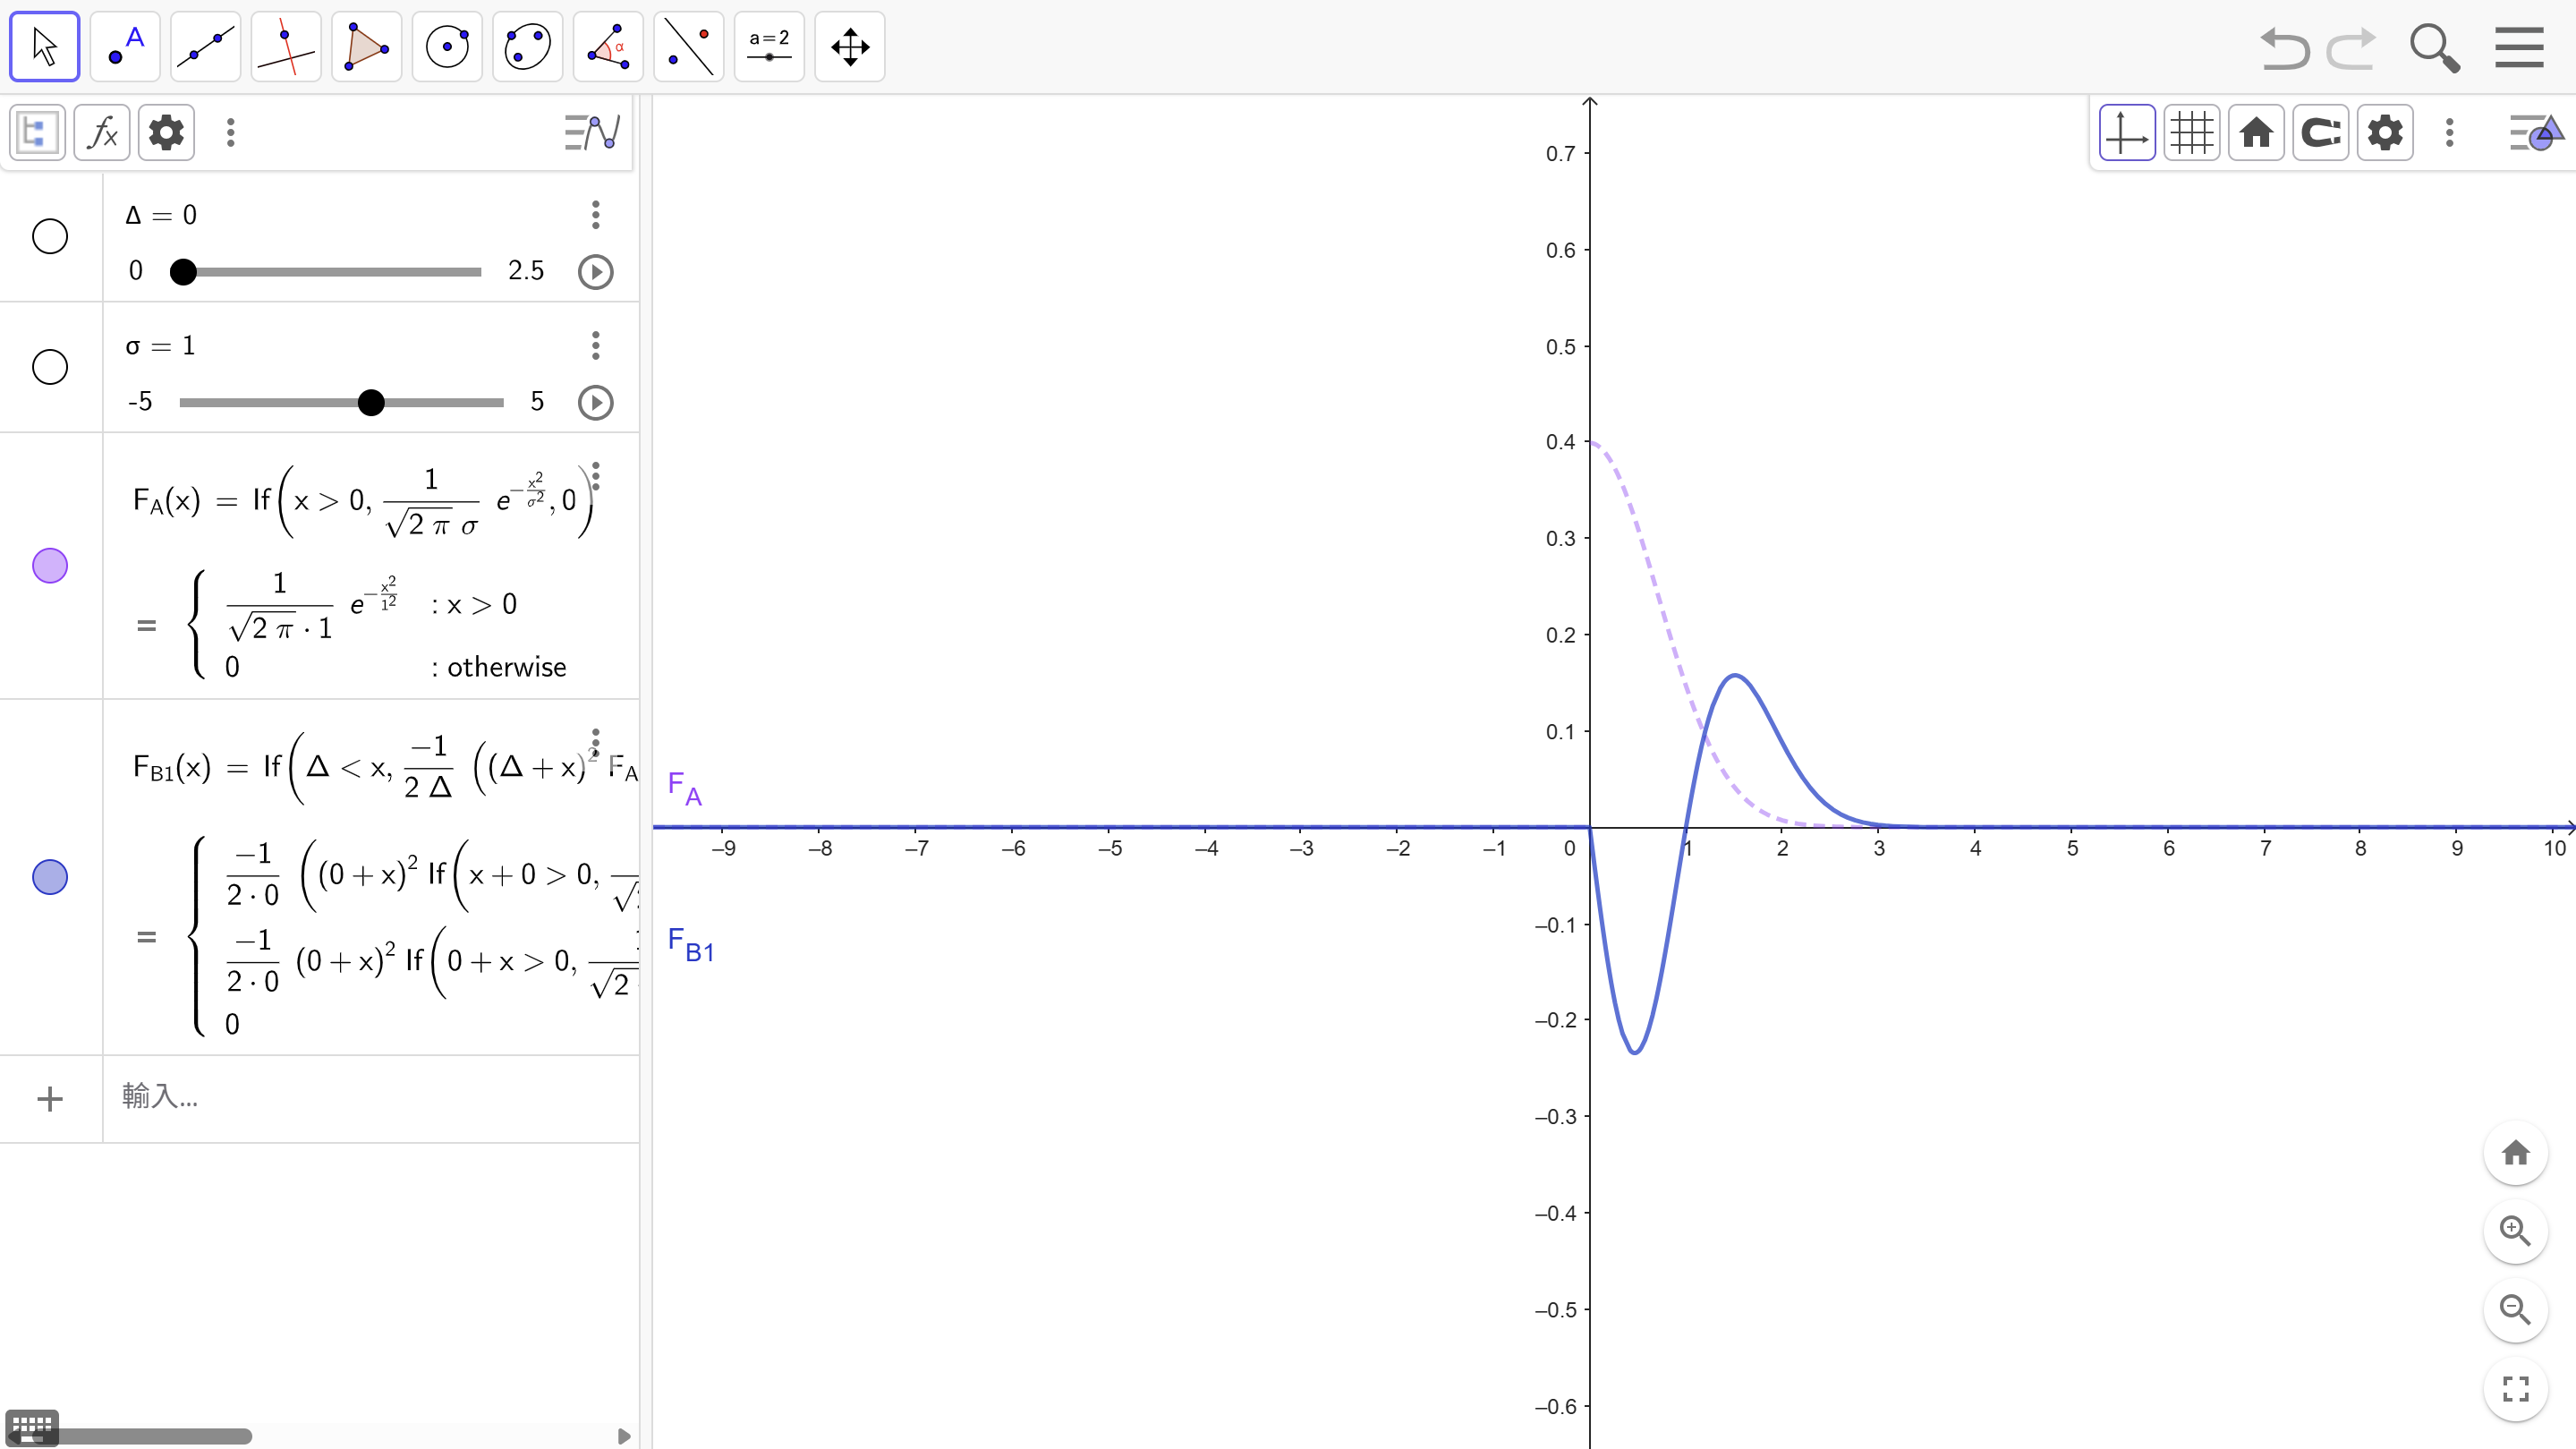
\includegraphics[width=\textwidth]{fig/Fa0.png}
         \caption{t $\rightarrow$ 0}
         \label{fig:t0}
    \end{subfigure}
    \hfill
    \begin{subfigure}[b]{0.4\textwidth}
         \centering
         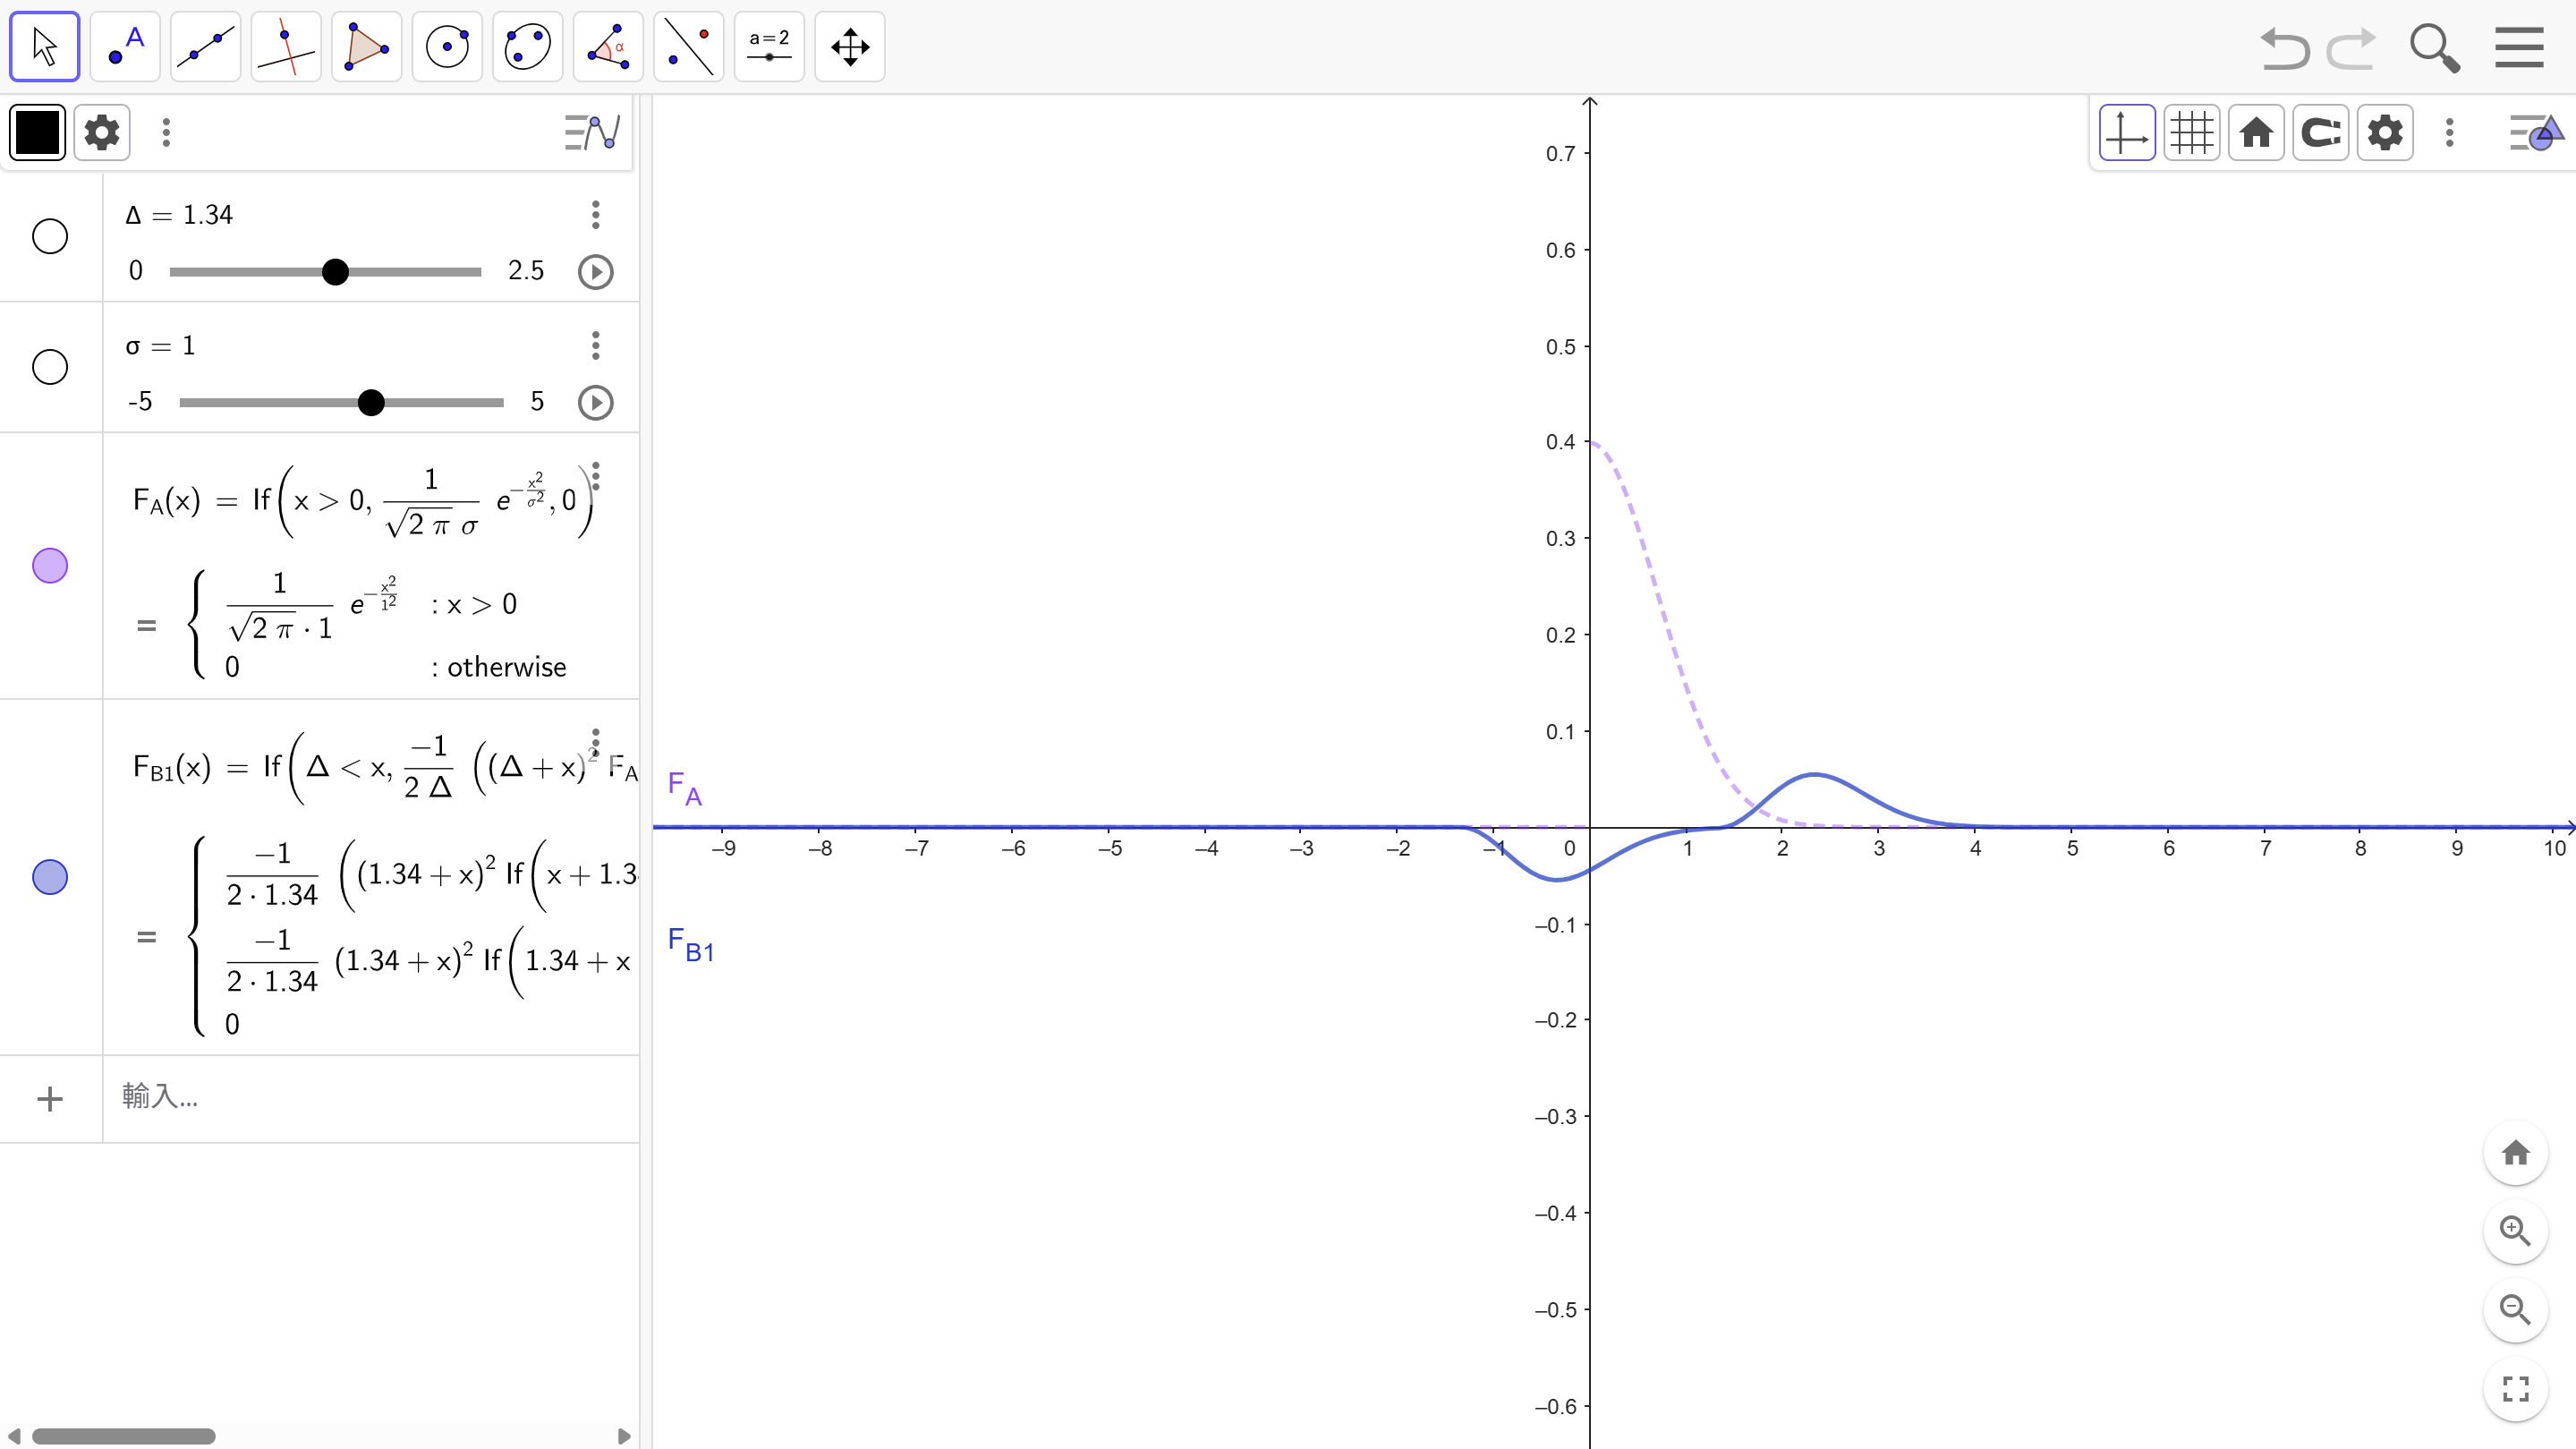
\includegraphics[width=\textwidth]{fig/Fa1.png}
         \caption{t = 1.34}
         \label{fig:t1}
    \end{subfigure}
    \hfill
    \begin{subfigure}[b]{0.4\textwidth}
         \centering
         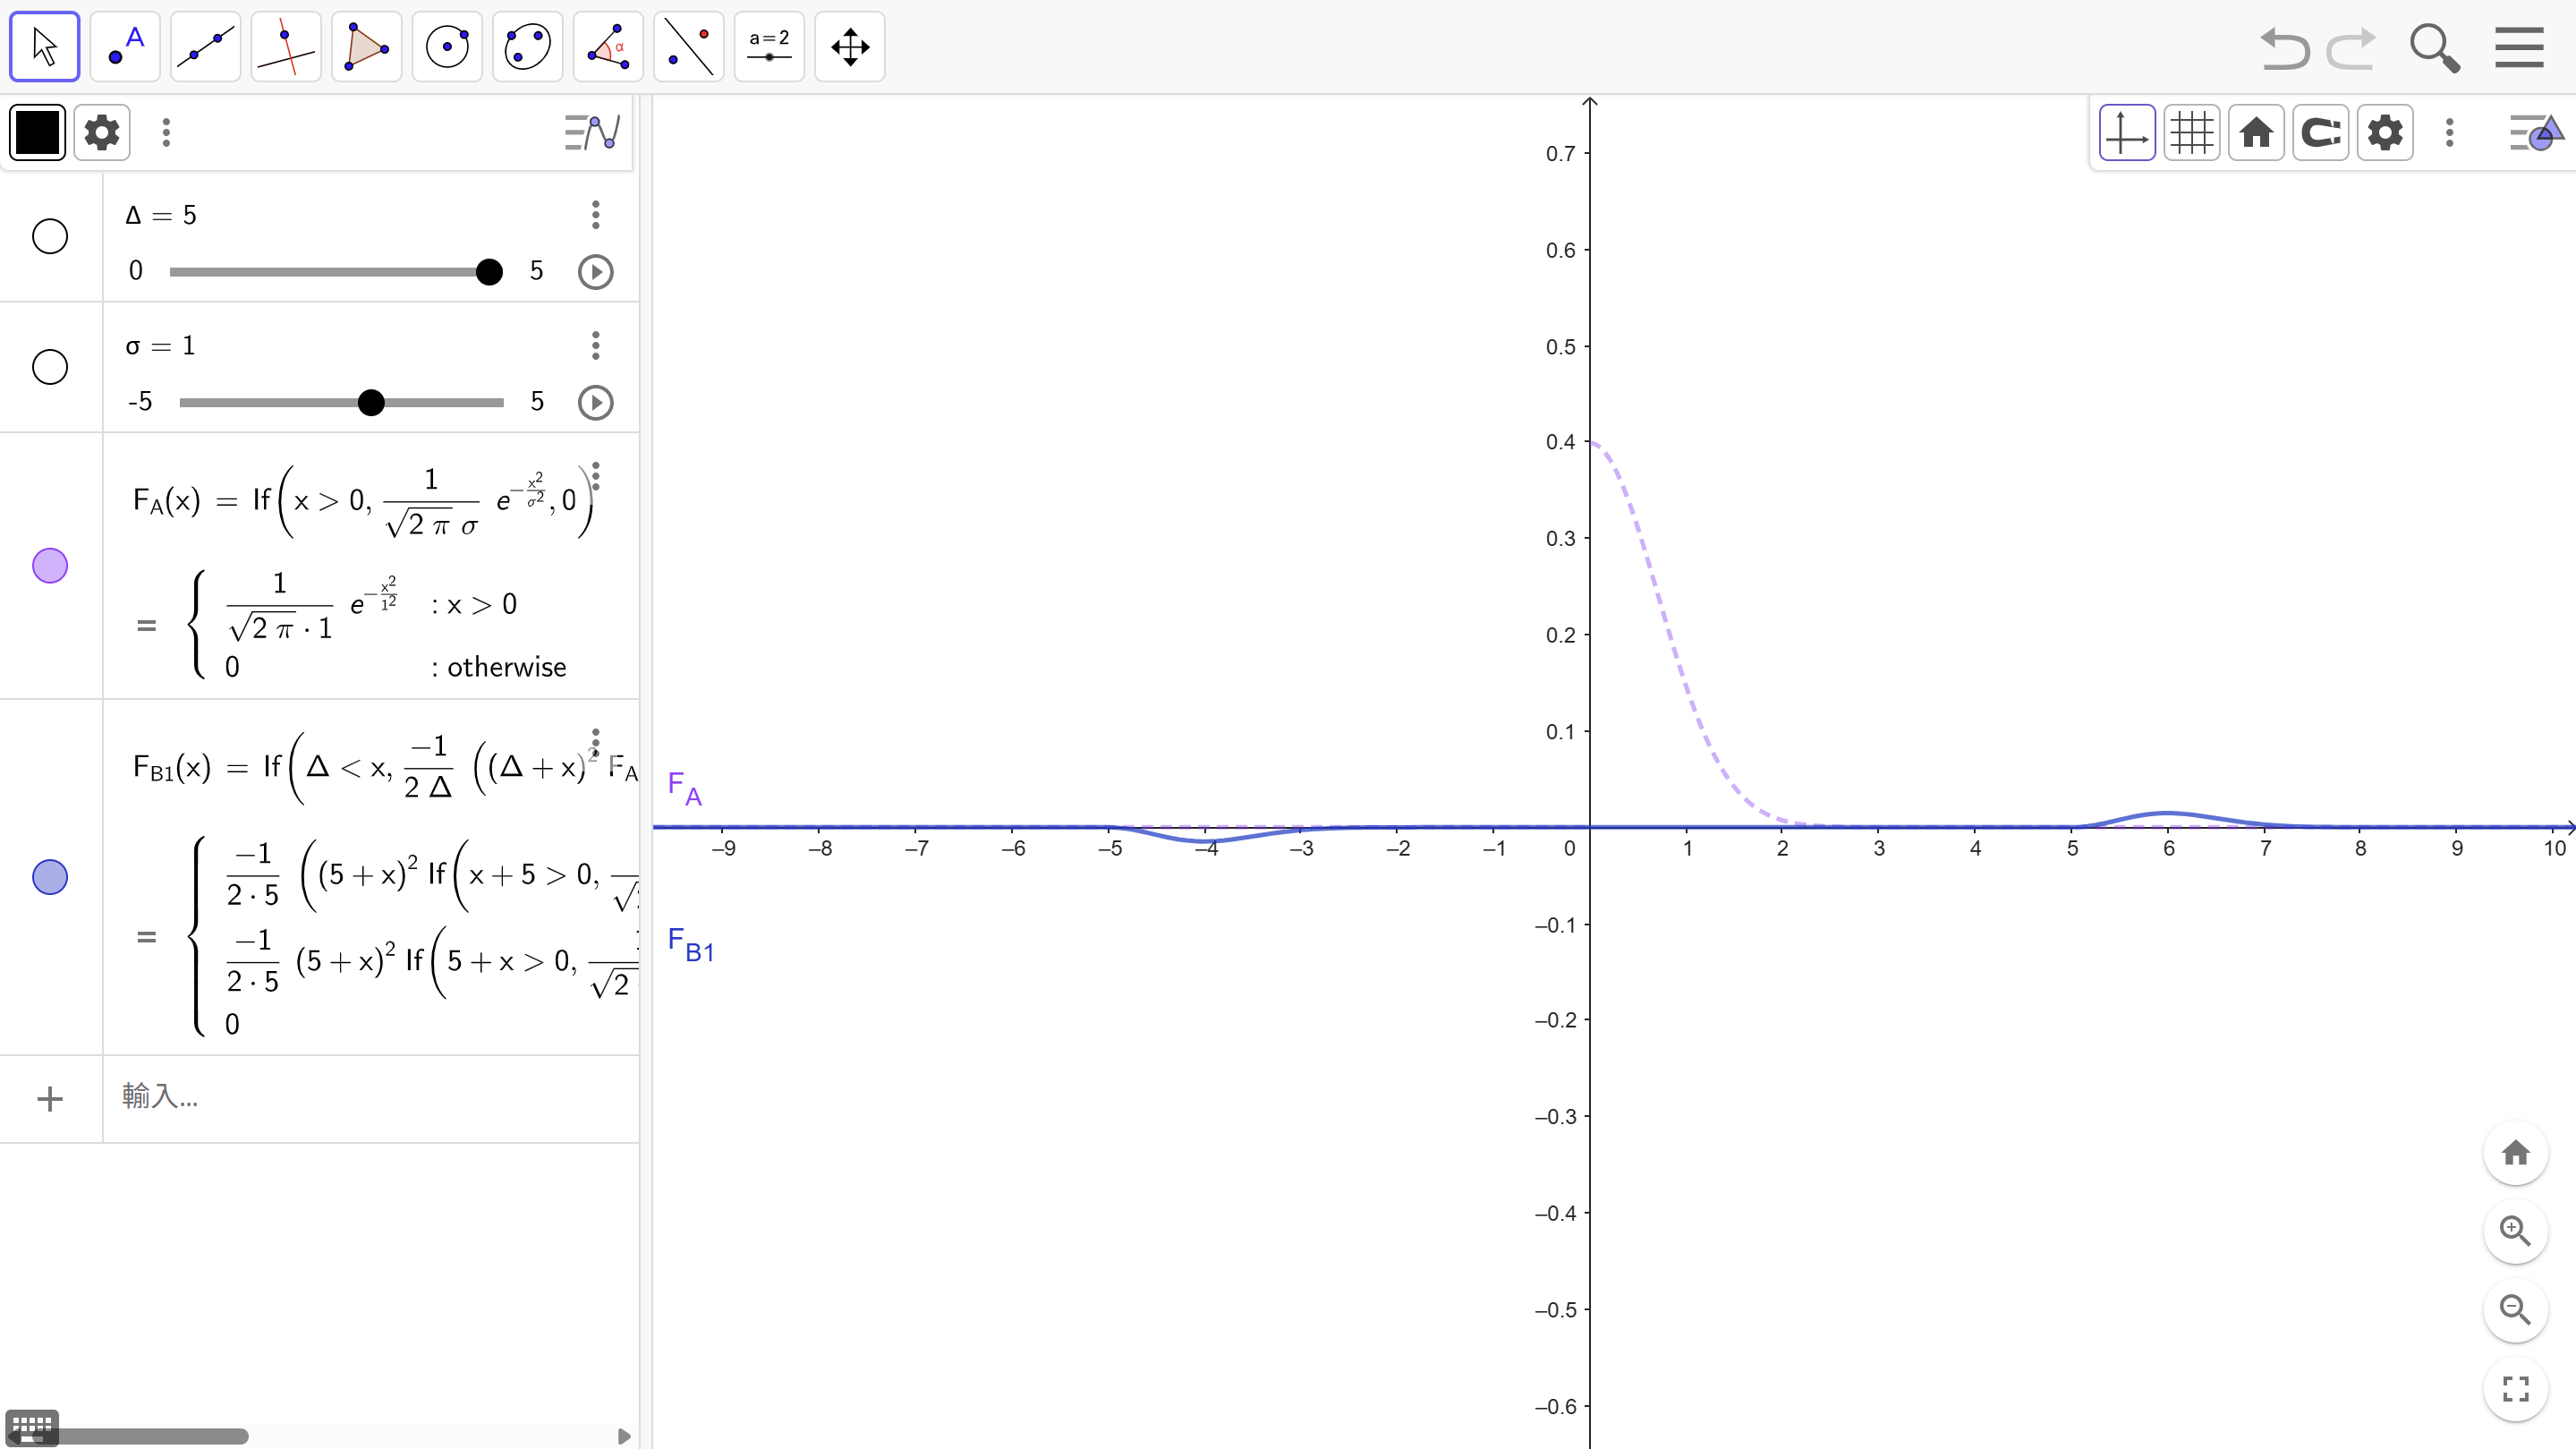
\includegraphics[width=\textwidth]{fig/Fa2.png}
         \caption{t = 5}
         \label{fig:t2}
    \end{subfigure}
\end{figure}
From the figures above, we can observe that the propagation of $F_{B1}$ does not exhibit any non-isotropic behavior. The distribution remains symmetric along the axis, indicating that the chosen smearing function, despite being non-isotropic, does not lead to anisotropic propagation in this setup.

It is similar to calculate \(F_{B2}, F_{B3}\), we could explicitly write out what they are, 
\begin{equation}
    F_{B2}(\mathbf{x}) = - \int \mathrm{d}\theta\, \delta(\theta)  \int \mathrm{d}\phi\, \int \mathrm{d}r\, r^2 \, R(r) \frac{\delta '\left(\sqrt{r^2 + x^2 - 2rx \cos\gamma} - \Delta\right)}{4\pi \sqrt{r^2 + x^2 - 2rx \cos\gamma}} \notag \\
\end{equation}
\begin{equation}
    F_{B3}(\mathbf{x}) = - \int \mathrm{d}\theta\, \delta(\theta)  \int \mathrm{d}\phi\, \int \mathrm{d}r\, r^2 \, R(r) \frac{\delta ''\left(\sqrt{r^2 + x^2 - 2rx \cos\gamma} - \Delta\right)}{4\pi \sqrt{r^2 + x^2 - 2rx \cos\gamma}} \notag \\
\end{equation}
where \(\displaystyle \delta '(x) = \frac{d \delta(x)}{d x}\) and \(\displaystyle \delta '''(x) = \frac{d^2 \delta(x)}{d x^2}\). Note that is derivative is differential over x, in the original equation, it becomes differentialing over \(\sqrt{r^2 + x^2 - 2rx \cos{\gamma}}\). Thus we need to do a change of variable, Chain rule, to change the variable to \(r\). After these messy calculation, we obtain the following equations
\begin{equation}
    F_{B2}(\mathbf{x}) = \int \frac{1}{\Delta}\left(\delta '(r - r_+) + \delta '(r - r_-) \right)g(r) r^2 R(r) \mathrm{d} r 
\end{equation}
\begin{equation}
    F_{B3}(\mathbf{x}) = \int \frac{1}{\Delta}\left(g(r) (\delta '(r - r_+) + \delta '(r - r_-)) \right) g(r) r^2 R(r) \mathrm{d} r 
\end{equation}
where \(g(r) = \frac{d r}{d \sqrt{r^2 + x^2 - 2rx \cos{\gamma}}}\).
By using the following properties of Dirac delta function,
\begin{align}
    &\int \mathrm{d} x \, \delta '(x-a) f(x) = f'(a)\\
    &\int \mathrm{d} x \, \delta ''(x-a) f(x) = f''(a)
\end{align}
we obtain 
\begin{align*}
    F_{B2}(\mathbf{x}) &= \frac{\Delta  (\Delta -x) e^{-\frac{(x-\Delta )^2}{\sigma ^2}} \left((x-\Delta )^2-\sigma ^2\right)}{\sqrt{\Delta ^2} \sigma ^2}\operatorname{sgn}(x - \Delta)\\ &+\frac{\Delta  (\Delta +x) e^{-\frac{(\Delta +x)^2}{\sigma ^2}} \left((\Delta +x)^2-\sigma ^2\right)}{\sqrt{\Delta ^2} \sigma ^2} \operatorname{sgn}(x + \Delta)
\end{align*}

{\footnotesize\begin{align*}
    F_{B3}(\mathbf{x}) &= \frac{e^{-\frac{(x-\Delta )^2}{\sigma ^2}} \left(-5 \Delta ^2 \sigma ^2+2 \Delta ^4+\sigma ^4+x^2 \left(12 \Delta ^2-5 \sigma ^2\right)-8 \Delta  x^3+2 x^4+x \left(10 \Delta  \sigma ^2-8 \Delta ^3\right)\right)}{\sigma ^4}\operatorname{sgn}(x - \Delta)\\
    &+\frac{e^{-\frac{(\Delta +x)^2}{\sigma ^2}} \left(-5 \Delta ^2 \sigma ^2+2 \Delta ^4+\sigma ^4+x^2 \left(12 \Delta ^2-5 \sigma ^2\right)+8 \Delta  x^3+2 x^4+2 x \left(4 \Delta ^3-5 \Delta  \sigma ^2\right)\right)}{\sigma ^4}\operatorname{sgn}(x + \Delta) 
\end{align*}}
The figure of both is plotted below, we can see that it is indeed surviving in the \(\theta = 0\) direction and \(\theta = \pi\) direction. Thus we can't make a isotropic quantum teleportation via this setup.

% \begin{figure}[htbp]
%     \centering
%     \subfigure[FB2]{
%         \includegraphics[width=0.45\textwidth]{FB2.pdf}
%         \label{fig:sub1}
%     }
%     \hfill
%     \subfigure[FB3]{
%         \includegraphics[width=0.45\textwidth]{FB3.pdf}
%         \label{fig:sub2}
%     }
%     \caption{Comparison of FB2 and FB3}
%     \label{fig:combined}
% \end{figure}

\appendix

\acknowledgments

% Bibliography

%% [A] Recommended: using JHEP.bst file
%% \bibliographystyle{JHEP}
%% \bibliography{biblio.bib}

%% or
%% [B] Manual formatting (see below)
%% (i) We suggest to always provide author, title and journal data or doi:
%% in short all the information that clearly identify a document.
%% (ii) please avoid comments such as "For a review'', "For some examples",
%% "and references therein" or move them in the text. In general, please leave only references in the bibliography and move all
%% accessory text in footnotes.
%% (iii) Also, please have only one work for each \bibitem.
\bibliographystyle{plain}
\bibliography{ref}

% Example reference entry in ref.bib
% @article{example_reference,
%   author = {Author Name},
%   title = {Example Title},
%   journal = {Example Journal},
%   year = {2023},
%   volume = {1},
%   pages = {1--10}
% }
\end{document}
